\chapter{Machine learning: an overview}
\label{chp:ml}
This chapter is dedicated to the theoretical exploration of the various models that have been used
in the project, I will start by considering supervised models, which represent the majority of the
models utilized, followed by a brief overview of the few unsupervised models used to extrapolate
more information from the data.
\section{The machine learning problem}
Before devling into the topic of the actual machine learning models I want to spend a few lines to
introduce the concept of 'machine learning problem', in the recent era, with the advent of ChatGPT
and other AI assistants I think the border of the various AI-related subjects has become fuzzier
than it already was in the beginning.

In the rest of the thesis I will be talking about machine learning, which is a subset of artificial
intelligence, and is a technique that allows one to solve complex problems without the constraints
of common problem-solving \cite{Rebala2019}. There are many different problems which solution is extremely hard to
explain in terms of a set of well-defined rules to be applied in order to go from the inputs to the
outputs, some easy examples that come to mind have usually to do with the classification of images:
\begin{itemize}
	\item Given a set of pictures of chihuahuas and muffins and taken one picture randomly,
	      having a classic algorithm that can tell us whether the picture is a chihuahua or a muffin,
	\item Given a set of pictures containing old women, having a classic algorithm that can tell
	      us whether a picture taken randomly is representing our grandma or not.
\end{itemize}
These examples can most likely be solved using image-processing techniques, but finding a solution
that can work reliably is going to take a lot of time and effort. A machine learning algorithm
allows us to abstract the complexity of the problem by allowing a model to find a pattern in our
dataset and then applying the newfound pattern to data that it has never seen.

\medskip

Therefore, whenever machine learning is applied to a certain problem the complexity of defining an
algorithm that can actually solve the problem is being exchanged with the complexity of finding a
model can can solve the problem reliably, and that can find a pattern that can be easily generalized
to other instances of the same problem.

In general, machine learning problems can be divided into two macrocategories: \emph{classification}
and \emph{regression}.

\smallskip

A regression problem is a problem that requires us to find the function that best \emph{fits} the
data at our disposal and therefore will be able to give us the best possible predictions for unknown
values. Very common regression problems are: Predicting the number of wins of a football team,
Projecting the price of a house on the market, Predicting the temperature of a certain country a
given number of years from now.

\smallskip

Classification problems, which are the ones that I will be considering in this chapter, can be
binary or multiclass, and require us to find the function that can, with the highest accuracy,
predict whether a certain datapoint belongs to a class or not. Some examples of binary
classification problems can be: Identifying whether a random picture is a Chihuahua or a Muffin,
Predicting whether there will be rain or not, Classifying an event as 'quench' or 'non-quench'.

\medskip

Since the problem at hand as a high grade of difficulty due to the amount of physics involved, for
the rest of this chapter, whenever an example is going to be needed to clarify a concept, I am going
to refer to the more accessible binary classification problem of 'Is it going to rain today?'
\section{Supervised models}
In the following we consider a dataset $\dset$ to be a set of pairs
in which $x_i$ are called \emph{features} and $y_i$ are called \emph{labels}. Labels, in the context
of binary classification, represent the answer, 'Yes' or 'No', 'True' or 'False'; features are a set of
values (numerical or other) that characterize the domain of the problem. In the context of our mock-problem, while
labels represent whether on day $k$ it rained or not, features could be a series of meteorological
information measured on day $k$ (e.g. humidity in the air, temperature, season, percentage of UV
exposure\ldots).

The problem that this thesis aims to solve is particularly suited for the application of supervised
models since the data at our disposal had already been labelled in previous works
\cite{mariotto2022-generic} \cite{mariotto2022}.

Before introducing theoretically the various models that have been used to solve the problems at
hand I want to introduce two very important issues in the field of supervised machine learning.
Let's suppose that we have at our disposal a dataset $\dset$, this dataset contains information
about the last year, for every day it's known whether it rained or not. Independently of the kind of
split taken to divide train and test dataset (let's suppose that the class distribution remains
unaltered between test and train datasets), let's now suppose that we have at our disposal two
different models: model $M_1$ has an accuracy of $100\%$ on the training set and an accuracy of
$93\%$ on the test set, model $M_2$ has an accuracy of $92\%$ on the training set and an accuracy of
$91\%$ on the test set.

Independently of other metric measures (which are not useful for this specific example), which model
would we rather take?

Model $M_1$ is clearly suffering from \emph{overfitting}, this means that it's not abstracting
enough from the training data and the result is that it's actually \emph{learning} the data, this is
undoubtedly a bad practice because when the model learns the data instead of a pattern therein
contained it's going to have very poor generalization performance.

An 'orthogonal' problem to overfitting is the issue of \emph{underfitting}, which is usually caused
by a model not being powerful enough to abstract information from a certain dataset.

In the following I will be discussing on a theoretical level the various supervised models deployed
to solve the problem.
\subsection{Decision Trees}
Decision Trees, implemented in the \emph{DecisionTreeClassifier} class of scikit-learn are amongst the
simplest and most effective machine learning models at our disposal. These models have a tree
structure and in every internal node a logical condition is evaluated on a subset of the features
in the dataset, while leaves contain the classification outcome.

One of the most important characteristics of the decision tree model is its high grade of
explainability, if we take the simple model built on the example in \cref{fig:simple-dt}, we can say
that to reliably describe a rainy day all is necessary is a coefficient of humidity of at least
$80\%$ and an outside temperature of at least $10C$.
\begin{figure}
	\centering
	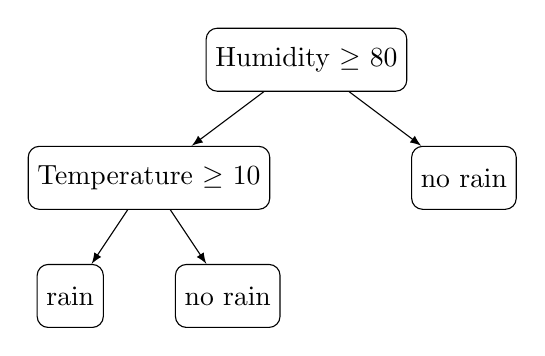
\begin{tikzpicture}[
			% Define styles for nodes
			level 1/.style={sibling distance=40mm},
			level 2/.style={sibling distance=20mm},
			level 3/.style={sibling distance=10mm},
			every node/.style={draw, rectangle, rounded corners, align=center, minimum size=8mm},
			edge from parent/.style={draw, -latex}
		]

		% Root node
		\node {Humidity $\geq$ 80}
		% First level
		child {node {Temperature $\geq$ 10}
				% Second level
				child {node {rain}}
				child {node {no rain}}
			}
		child {node {no rain}};
	\end{tikzpicture}
	\caption{A very simple example of decision tree built on the mock problem}
	\label{fig:simple-dt}
\end{figure}
\subsection{Random Forests}
\subsection{SVM}
\section{Unsupervised models}
\subsection{Clustering with k\-means}
